\documentclass[14pt]{article}

\usepackage[margin=1.5cm]{geometry}
\usepackage{enumerate}
\usepackage{amsmath,amssymb}
\usepackage{tikz}

\begin{document}

\begin{center}
Proficiency Exam 3 - Linear Transformations
\end{center}

You will have 30 minutes to complete the exam.  You may use a calculator, but you must show all steps done to get full credit for completing the problem.  This means that if you use your calculator for anything other than arithmetic, you must indicate on your test paper what you did on the calculator.

\begin{enumerate}
\item Is the function $ F \colon \mathbb{R}^2 \rightarrow \mathbb{R}^3 $ given by
\[
F(x_1,x_2) = \left[\begin{array}{c}x_1+x_2 \\ x_1-x_2 \\ 2x_1-3x_2\end{array}\right]
\]
a linear transformation?  If it is, prove it.  If it isn't, provide a counterexample that shows it is not.

\item Find the matrix representation of the linear transformation pictured below.
\begin{center}
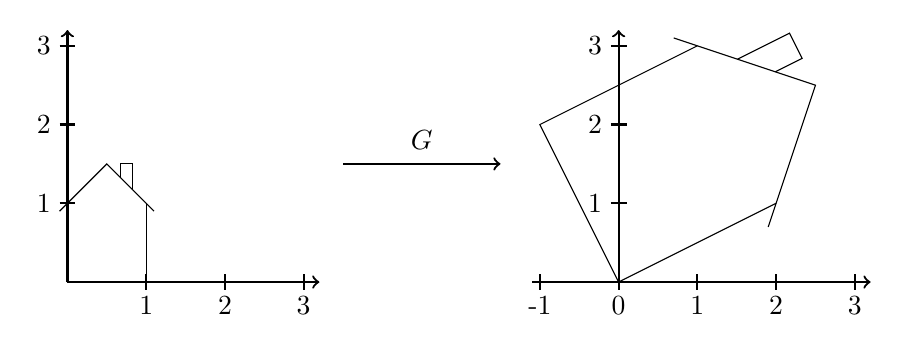
\begin{tikzpicture}
\draw[->,thick] (0,0) -- (0,3.2);
\draw[->,thick] (0,0) -- (3.2,0);
\draw[thick] (1,-0.1) -- (1,0.1);
\node at (1,-0.3) {1};
\draw[thick] (2,-0.1) -- (2,0.1);
\node at (2,-0.3) {2};
\draw[thick] (3,-0.1) -- (3,0.1);
\node at (3,-0.3) {3};
\draw[thick] (-0.1,1) -- (0.1,1);
\node at (-0.3,1) {1};
\draw[thick] (-0.1,2) -- (0.1,2);
\node at (-0.3,2) {2};
\draw[thick] (-0.1,3) -- (0.1,3);
\node at (-0.3,3) {3};

\draw (-0.1,0.9) -- (0.5,1.5) -- (1.1,0.9);
\draw (1,0) -- (1,1);
\draw (0.67,1.33) -- (0.67,1.5) -- (0.83,1.5) -- (0.83,1.17);

\draw[->,thick] (3.5,1.5) -- (5.5,1.5);
\node at (4.5,1.8) {$G$};

\draw[->,thick] (7,-0.1) -- (7,3.2);
\draw[->,thick] (5.9,0) -- (10.2,0);
\draw[thick] (6,-0.1) -- (6,0.1);
\node at (6,-0.3) {-1};
\node at (7,-0.3) {0};
\draw[thick] (8,-0.1) -- (8,0.1);
\node at (8,-0.3) {1};
\draw[thick] (9,-0.1) -- (9,0.1);
\node at (9,-0.3) {2};
\draw[thick] (10,-0.1) -- (10,0.1);
\node at (10,-0.3) {3};
\draw[thick] (6.9,1) -- (7.1,1);
\node at (6.7,1) {1};
\draw[thick] (6.9,2) -- (7.1,2);
\node at (6.7,2) {2};
\draw[thick] (6.9,3) -- (7.1,3);
\node at (6.7,3) {3};
%\node at (6.7,0) {0};
%\node at(6.7,-1) {-1};
%\draw[thick] (6.9,-1) -- (7.1,-1);


%\draw (9,-1) -- (7,0) -- (8,2) -- (10,1);
%\draw (8.9,-1.1) -- (10.5,-0.5) -- (9.9,1.1);
%\draw (10.1,0.67) -- (10.8,0.4) -- (10.7,0.07) -- (10.2,0.25);
\draw (8,3) -- (6,2) -- (7,0) -- (9,1);
\draw (7.7,3.1) -- (9.5,2.5) -- (8.9,0.7);
\draw (8.99,2.67) -- (9.33,2.84) -- (9.17,3.16) -- (8.51,2.83);
\end{tikzpicture}
\end{center}

\item (TRUE or FALSE) Consider the statement and decide if it is true or false.  If true, provide reasoning.  If false, provide a counterexample.
\begin{center}
``If $ T\colon \mathbb{R}^m \rightarrow \mathbb{R}^n $ is onto, then $ m \leq n $."
\end{center}

\item  Is the following linear transformation onto?
\[
T(x_1,x_2,x_3) = \left[\begin{array}{c} x_1-3x_3 \\ 2x_2+4x_3 \\ -x_1 +3x_2+7x_3\end{array}\right]
\]






\end{enumerate}

\end{document}